\section{Tipos de Ciclos}

A eficiência avalia quão bem um sistema/ciclo converte a energia que é preciso fornecer ao sistema, indispensável para o seu funcionamento, no trabalho que se pretende obter, ou, no caso do rendimento de ciclos frigoríficos e bombas de calor, em quantidade de energia na forma de calor que se pretendia mover.

\begin{equation*}
    \eta = \frac{\text{``o que eu quero''}}{\text{``o que é preciso fornecer''}}
\end{equation*}

\subsection{Ciclo Motor}

Os ciclos motor têm como objetivo realizar trabalho, sendo preciso fornecer energia, normalmente sobre a forma de calor.
É preciso fornecer $Q_H$ para realizar $W_u$ e acabando inevitavelmente por ceder $Q_C$. Fazendo o balanço energético tem-se: $\Delta E = Q_H - W_u - Q_C$. Como se trata de um ciclo $\Delta E = 0$, pelo que $W_u = Q_H - Q_C$.

Portanto, a \textbf{eficiência térmica} de um ciclo motor é:

\begin{equation}
    \eta = \frac{W_u}{Q_H} = \frac{Q_H - Q_C}{Q_H}  = 1 - \frac{Q_C}{Q_H}
\end{equation}

onde $Q_H$ é a energia recebida pelo reservatório quente (combustível, radiação solar, reação nuclear controlada) e $Q_C$ a energia cedida ao reservatório frio. É claro que $Q_H > Q_C$ num ciclo motor, pois pretende-se que $W_u > 0$. Pela conservação da energia, a eficiência é $\eta \leq 1$. Se $Q_C = 0$, a eficiência térmica seria $100\%$, mas isto viola a Formulação de Kelvin-Planck. Assim, para o ciclo funcionar, parte do calor recebido $Q_H$ é obrigatoriamente transferido para a fonte fria, $Q_C$. Logo, $\eta < 1$, não havendo eficiências de $100\%$.
Esta conclusão pode ser considerado um \textbf{corolário da Segunda Lei da Termodinâmica}.

\subsubsection{Corolários de Carnot}

Outros dois corolários da Segunda Lei são conhecidos como Corolários de Carnot:

\begin{enumerate}
    \item A eficiência térmica de um processo irreversível é sempre menor que a eficiência térmica de um processo reversível, quando ambos operam entre os mesmos reservatórios.
    \item Todos os processos reversíveis a operar entre os mesmos dois reservatórios têm a mesma eficiência térmica.
\end{enumerate}

\begin{proof}
    Para demonstrar o primeiro corolário, basta considerar dois ciclos: um reversível R e o outro irreversível I a operar entre os mesmos dois reservatórios. Ambos recebem $Q_H$ e realizam trabalho $W_R$ e $W_I$. Pelo princípio da conservção da energia, ambos cedem calor ao reservatório frio igual a $Q_C = Q_H - W_R$ e $Q_C' = Q_H - W_I$. Considerando agora que o ciclo R opera no sentido contrário, e dado ser reversível as transferências de calor e trabalho mantém-se iguais, mas em sentido contrário. Desta forma, o reservatório quente mantém todas as suas propriedades, dado que recebe $Q_H$ de R e cede $Q_H$ a I. Assim, consideremos o sistema que engloba os dois ciclos e o reservatório quente, como cada parte deste sistema opera num ciclo ou não sofre alterações, então o sistema conjunto opera num ciclo. Além disso, este sistema troca calor com um único reservatório, pelo que, de acordo com Kelvin-Planck, $\oint \delta W > 0$, sendo irreversível, pois na sua operação pelo menos uma das suas partes é irreversível, o ciclo I. Desta forma, $W_R - W_I > 0 \Longleftrightarrow W_R > W_I$. Como ambos os ciclos inicialmente considerados recebem a mesma quantidade de energia, $Q_H$, $\eta_R > \eta_I$.
    O segundo corolário pode ser demosntrado igualmente para dois ciclos reversíveis. O ciclo conjunto é reversível, pelo que a igualdade de Kelvin-Planck é válida. Logo, $W_{R_1} = W_{R_2}$, e $\eta_{R_1}= \eta_{R_1}$ 
\end{proof}


\subsection{Ciclo Frigorífico e Bombas de Calor}

Nos ciclos frigoríficos ou bombas de calor, o sistema recebe $Q_C$ e $W_{\text{ciclo}}$, de modo a ceder $Q_H$, tal que $Q_H = Q_C + W_{\text{ciclo}}$, no caso ideal. Temos, então: $\Delta E = Q_C + W_{\text{ciclo}} - Q_H \implies W_{\text{ciclo}} = Q_H - Q_C$. Como é necessário fornecer trabalho $W_{\text{ciclo}} > 0$, então: $Q_H > Q_C$, novamente.

\subsubsection{Ciclo Frigorífico}

Um Ciclo Frigorífico tem como objetivo arrefecer um dado espaço. Por isso, o rendimento de um Ciclo Frigorífico, ou em inglês, \textit{coefficient of performance} (COP), é a razão entre o calor que se pretende remover da fonte fria (o frigorífico), e o trabalho que se teve de fornecer (e.g. energia elétrica).

\begin{equation}
    \text{COP}_{\text{frig.}} = \beta = \frac{Q_C}{W_{\text{ciclo}}} = \frac{Q_C}{Q_H - Q_C}
\end{equation}

\begin{equation}
    \beta = \frac{Q_C}{Q_H - Q_C} = \frac{Q_H - Q_H + Q_C}{Q_H - Q_C} = \frac{Q_H}{Q_H - Q_C} - 1 = \frac{1}{1 - \frac{Q_C}{Q_H}} - 1 = \frac{1}{\eta} - 1
\end{equation}

Assim, temos $\beta > 0$ e mostrámos que existe uma relação entre o rendimento do ciclo frigorífico e a eficiência do ciclo motor que se obtém invertendo a direção de operação do ciclo, entre os mesmos reservatórios.

\subsubsection{Bomba de Calor}

Na Bomba de Calor, o objetivo é transferir calor, $Q_H$, para um dado espaço, seja para manter uma habitação a uma temperatura superior à temperatura ambiente, seja em processos industriais. Por isso, o rendimento de uma Bomba de Calor é dado por:

\begin{equation}
    \text{COP}_{\text{bomba}} = \gamma = \frac{Q_H}{W_{\text{ciclo}}} = \frac{Q_H}{Q_H - Q_C}
\end{equation}

Se o trabalho que é necessário fornecer a uma Bomba de Calor (ou a um Ciclo Frigorífico), $W_{\text{ciclo}}$, aproximar-se de zero, o rendimento aproximar-se-ia de infinito. No entanto, se $W_{\text{ciclo}} = 0 \implies Q_H = Q_C$, pelo que o sistema iria tirar energia do reservatório frio e tranferi-la para o reservatório quente, espontaneamente -- pois nenhum trabalho foi fornecido --, o que viola a Formulação de Clausius.

Além disso, 

\begin{equation*}
    \gamma = \frac{Q_H}{Q_H - Q_C} = \frac{1}{1 - \frac{Q_C}{Q_H}}
\end{equation*}

pelo que $Q_H > Q_C \implies 0 < \frac{Q_C}{Q_H} < 1 \Longleftrightarrow 0 < 1 - \frac{Q_C}{Q_H} < 1 \implies \gamma > 1$.
Além disso, 

\begin{equation}
    \gamma = \frac{1}{\eta}
\end{equation}

i.e. o rendimento da Bomba de Calor é o inverso da eficiência do Ciclo Motor para o mesmo ciclo de processos a operar no sentido contrário entre os mesmos reservatórios. Caso a Bomba de Calor seja reversível, o seu rendimento é igual ao rendimento de qualquer outra Bomba de Calor reversível a operar entre os mesmos reservatórios e maior do que o rendimento de qualquer ciclo irreversível a operar entre os mesmos reservatórios.

Assim, os Corolários de Carnot também são válidos para os ciclos frigoríficos e bombas de calor, bastando, para isso, substituir o termo \textit{eficiência térmica} por \textit{rendimento}.


\subsection{Escala de Kelvin}

Do segundo corolário de Carnot, sabemos que quaisquer dois ciclos a operar entre os mesmos dois reservatórios têm a mesma eficiência térmica, sendo, portanto, independente dos processos internos de cada ciclo. Portanto, a eficiência térmica está apenas relacionada com a natureza dos reservatórios. Como é a diferença de temperatura que permite as trocas de calor e a produção de trabalho, concluimos que a eficiência térmica depende apenas das temperaturas dos reservatórios.

\begin{equation}
    \left( \frac{Q_C}{Q_H} \right)_{rev} = f(T_C, T_H)
\end{equation}

Esta equação pode ser usada como base para definir uma escala de temperatura, independente das propriedades da substância. A Escala de Kelvin foi definida então para $f = \frac{T_C}{T_H}$: 

\begin{equation}
    \left( \frac{Q_C}{Q_H} \right)_{rev} = \frac{T_C}{T_H}
\end{equation}

Assim, se um ciclo operar entre um reservatório a $273.16 K$ (temperatura do ponto triplo da água) e outra a uma temperatura $T$,

\begin{equation*}
    T = 273.16 \left( \frac{Q}{Q_{pt}} \right)_{rev}
\end{equation*}

Desta forma, quando $Q \to 0$, também $T \to 0$, pelo que podemos concluir que o zero absoluto é a menor temperatura atingível na Escala de Kelvin, ou escala absoluta de temperatura.

\subsection{Eficiência de Carnot}

\subsubsection{Ciclo Motor}

\begin{equation}
    \eta_{max} = 1 - \frac{T_C}{T_H}
\end{equation}

Note-se que a eficiência aumenta com $T_H$ mais elevada e/ou $T_C$ mais baixa. No entanto, em ciclos motores, a redução de $T_C$ é geralmente limitada por restrições práticas, uma vez que temperaturas inferiores à ambiente requerem um sistema frigorífico.

Estas conclusões estão qualitativamente corretas para ciclos reais, irreversíveis. Muitas vezes, maximizar a eficiência térmica pode não ser o único objetivo. Considerações de custo e limitações físicas podem mostrar que uma eficiência de 40 \% pode não parecer assim tão pouco, relativamente a um valor limitante realista de 60\%, por exemplo, em vez de 100\%.

\subsubsection{Ciclo Frigorífico}

\begin{equation}
    \beta_{max} = \frac{T_C}{T_H - T_C}
\end{equation}

\subsubsection{Bomba de Calor}

\begin{equation}
    \gamma_{max} = \frac{T_H}{T_H - T_C}
\end{equation}

Note-se que as temperaturas têm de ser temperaturas absolutas na escala de Kelvin ou na de Rankine, pois são escalas absolutas que diferem de um fator multiplicativo: $T(\text{\textdegree R}) = 1.8 \, T(\text{K})$, enquanto as escalas de Celsius e Fahrenheit têm uma translação arbitrária em relação ao zero absoluto.


\subsection{Ciclo de Carnot}

Num Ciclo de Carnot, um sistema passa por quatro processos internamente reversíveis: dois \textbf{processos adiabáticos} alternados com dois \textbf{processos isotérmicos}.

Exemplo do Ciclo de Carnot para um sistema de gás num êmbolo-cilindro. As paredes do sistema são adiabáticas.

\begin{itemize}
    \item \textbf{Processo 1 $\rightarrow$ 2:} O sistema entra em contacto com o reservatório a $T_H$. O gás expande isotermicamente, enquanto recebe $Q_H$.
    \item \textbf{Processo 2 $\rightarrow$ 3:} O gás é permitido expandir adiabaticamente até a temperatura diminuir até $T_C$.
    \item \textbf{Processo 3 $\rightarrow$ 4:} O sistema entra em contacto com o reservatório a $T_C$. O gás comprime isotermicamente, cedendo $Q_C$.
    \item \textbf{Processo 4 $\rightarrow$ 1:} O gás é comprimido adiabaticamente até atingir $T_H$.
\end{itemize}

Para o Processo 1 $\rightarrow$ 2 ser reversível, a diferença entre a temperatura do gás e a temperatura do reservatório deve ser tendencionalmente nula. Desta forma, dado que o reservatório mantém a sua temperatura, implica que a temperatura do gás também deve ser constante. Idem, para o Processo 3 $\rightarrow$ 4.

Um Ciclo de Carnot a operar na direção contrária é um Ciclo Frigorífico ou uma Bomba de Calor. Um Ciclo de Carnot também pode ser composto por processos onde um condensador é carregado e descarregado, ou uma substância paramagnética é magnetizada ou desmagnetizada.

\subsubsection{Trabalho Compressão/Expansão}

Para um gás ideal, num sistema êmbolo-cilindro como descrito anteriormente, sabemos que o trabalho dos processos de compressão e expansão isotérmicos é dado por \ref{eq:trabalho-gas-ideal}:

\begin{equation}
    W = - mRT \ln \frac{V_2}{V_1} = - mRT \ln \frac{\frac{mR T}{p_2}}{\frac{mR T}{p_1}} = - mRT \ln \frac{p_1}{p_2} = mRT \ln \frac{p_2}{p_1}
\end{equation}

E, assim, podemos observar, no Ciclo de Carnot, que:

\begin{itemize}
    \item \textbf{Compressão ($p_2 > p_1$)}: é necessário arrefecer (ceder $Q_C$ no Processo 3 $\rightarrow$ 4) o sistema para diminuir a entropia e para diminuir o trabalho de compressão, pois $T \downarrow \implies W \downarrow$.
    \item \textbf{Expansão ($p_2 < p_1$)}: no Processo 1 $\rightarrow$ 2, pretende-se obter o máximo de calor, $Q_H$, para aumentar a temperatura do sistema, pois, quanto maior a temperatura, maior será o trabalho obtido na expansão ($T \uparrow \implies W \uparrow$).
\end{itemize}



\section{Ciclo de Carnot}

O Ciclo de Carnot pode ser aplicado a um um ciclo motor reversível com água circulante, onde $\nabla T, \nabla P \to 0$ e $\sigma = 0$, considerando \textbf{processos adiabáticos} na turbina e na bomba, e \textbf{processos isotérmicos} no condensador e na caldeira.

\begin{itemize}
    \item \textbf{Processo 1 $\rightarrow$ 2 (Caldeira):} A água passa do estado líquido ao gasoso isotermicamente, logo, a pressão constante, enquanto recebe $Q_H$.
    \item \textbf{Processo 2 $\rightarrow$ 3 (Turbina):} O vapor, que sai da caldeira, expande na turbina adiabaticamente, realizando trabalho. A temperatura diminui para $T_C$ e a pressão diminui.
    \item \textbf{Processo 3 $\rightarrow$ 4 (Condensador):} Algum vapor condensa isotermicamente a $T_C$, a pressão constante.
    \item \textbf{Processo 4 $\rightarrow$ 1 (Bomba):} A bomba recebe a mistura de duas fases do condensador e comprime adiabaticamente até $T_H$. 
\end{itemize}

\begin{figure}[H]
    \centering
    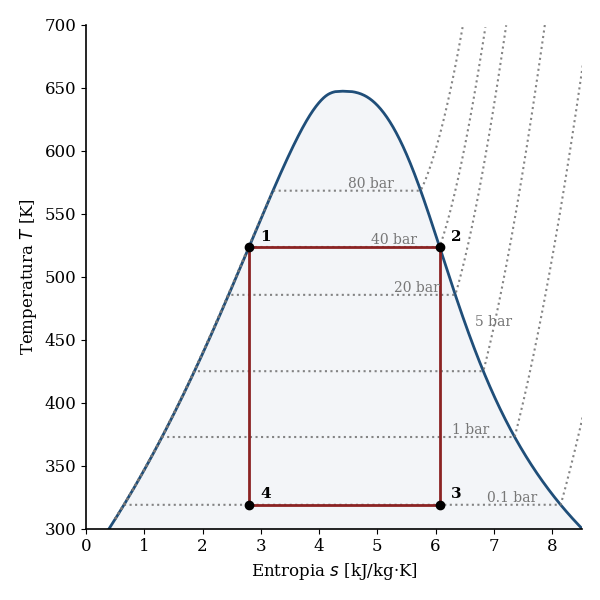
\includegraphics[width=0.45\linewidth]{graphs/carnot-Ts-ideal.png}
    \caption{Ciclo Carnot}
    \label{fig:carnot-Ts}
\end{figure}

Como se tratam de processos reversíveis, no contacto com os reservatórios: $ds = \frac{\delta Q}{T} + \delta \cancelto{0}{\sigma}$ e temos, então $\delta Q = T ds$. Logo, o valor do integral: $Q = \int T ds$, é igual ao calor total transferido no contacto com os reservatórios. Num diagrama T-s, este corresponde à área por baixo das linhas isotérmicas $T_H$ e $T_C$.

Fazendo os balanços de energia e entropia para cada processo, obtém-se:

\begin{itemize}
    \item \textbf{Processo 1 $\rightarrow$ 2 (Caldeira):} $\Delta U_{12} = Q_H - W_{12}$ e $\Delta S_{12} = \frac{Q_{H}}{T_H}$
    \item \textbf{Processo 2 $\rightarrow$ 3 (Turbina):} $\Delta U_{23} = -W_{23}$ e $\Delta S_{23} = 0$
    \item \textbf{Processo 3 $\rightarrow$ 4 (Condensador):} $\Delta U_{34} = -Q_C + W_{34}$ e $\Delta S_{34} = - \frac{Q_{C}}{T_C}$
    \item \textbf{Processo 4 $\rightarrow$ 1 (Bomba):} $\Delta U_{41} = W_{41}$ e $\Delta S_{41} = 0$
\end{itemize}

Como se trata de um ciclo $\Delta U = 0$, então:
\begin{equation*}
    \sum_i \Delta U_i = \sum_i Q_i + \sum_i W_i \Longleftrightarrow 0 = Q_H - Q_C - W_{12} - W_{23} + W_{34} + W_{41}
\end{equation*}

Portanto, o trabalho útil do ciclo é:

\begin{equation}
    W_u = W_{12} + W_{23} - ( W_{34} +  W_{41}) = Q_H - Q_C
\end{equation}

Ou, de outra forma, o trabalho do ciclo é $W_u = \int T_H ds + \int T_C ds = T_H \Delta S_{12} +  T_C \Delta S_{34} = Q_H - Q_C$.


No ciclo, $\sum_i \Delta S_i = 0 \Longleftrightarrow \Delta S_{12} + \Delta S_{34} = 0 \Longleftrightarrow \frac{Q_H}{T_H} - \frac{Q_C}{T_C} = 0 \implies \frac{Q_C}{Q_H} = \frac{T_C}{T_H}$. E, novamente,

\begin{equation}
    \eta_{rev} = 1 - \frac{Q_C}{Q_H} = 1 - \frac{T_C}{T_H}
\end{equation}

\begin{examplebox}[Ciclos Reversíveis]

O trabalho do ciclo $W_u = \int T_H ds + \int T_C ds $ pode ser generalizado para qualquer ciclo reversível, onde o trabalho útil do ciclo será a área contida entre as linhas dos processos do ciclo.

\begin{figure}[H]
    \centering
    \begin{subfigure}{0.32\textwidth}
        \centering
        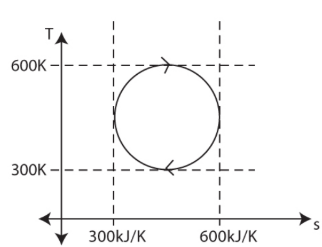
\includegraphics[width=\textwidth]{images/ciclo-circulo.png}
        \caption{Ciclo reversível - círculo}
        \label{fig:rev-circulo}
    \end{subfigure}
    \hfill
    \begin{subfigure}{0.62\textwidth}
        \centering
        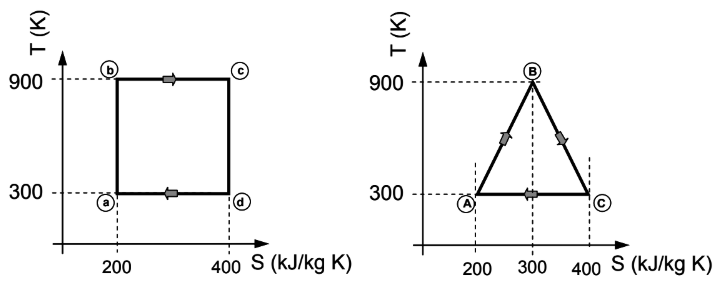
\includegraphics[width=\textwidth]{images/ciclos-triangulo.png}
        \caption{Quadrado (Carnot) e Triângulo}
        \label{fig:rev-triangulo}
    \end{subfigure}
    \caption{Exemplos de ciclos reversíveis}
\end{figure}

\begin{itemize}
    \item Círculo: $W_u = \text{``área do círculo''} = \pi \cdot 150^2$ (kJ)
    \item Quadrado: $W_u = T_H \Delta S_{bc} + T_C \Delta S_{da} = 900\cdot(400-200) + 300\cdot (200 -400) = 120000~\text{kJ/kg}$\\
                    ou $W_u = \text{``área do quadrado''} = (900 - 300)\cdot(400-200)= 120000~\text{kJ/kg}$
    \item Triângulo: $W_u = (400-200) \cdot (900 -300) /2 = 60000~\text{kJ/kg}$
\end{itemize}

\end{examplebox}


\subsection{Ciclo Motor Real}

Num ciclo real, quando o sistema entra em contacto com o reservatório a $T_H$, o sistema está a $T_H' < T_H$, e, quando entra em contacto com o reservatório a $T_C$, encontra-se a $T_C' > T_C$, tal como representado na Figura \ref{fig:ciclo-real}.

\begin{figure}[H]
    \centering
    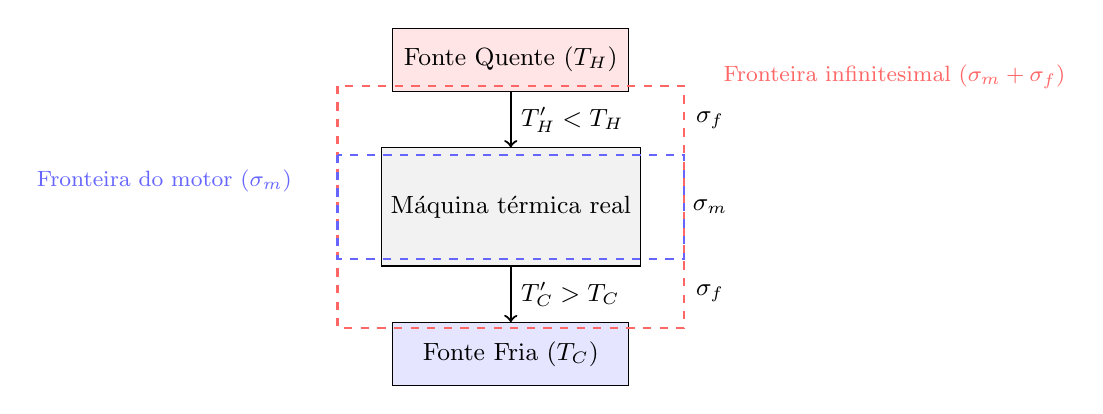
\begin{tikzpicture}[scale=1.1, every node/.style={font=\small}]
        % Heat reservoirs
        \node[draw, minimum width=3cm, minimum height=0.8cm, fill=red!10] (TH) at (0,3.4) {Fonte Quente ($T_H$)};
        \node[draw, minimum width=3cm, minimum height=0.8cm, fill=blue!10] (TC) at (0,0) {Fonte Fria ($T_C$)};
        
        % Heat engine
        \node[draw, minimum width=3cm, minimum height=1.5cm, fill=gray!10] (engine) at (0,1.7) {Máquina térmica real};

        % Arrows
        \draw[->, thick] (TH.south) -- node[right] {$T_H' < T_H$} (engine.north);
        \draw[->, thick] (engine.south) -- node[right] {$T_C' > T_C$} (TC.north);

        % Entropy labels
        \node at (2.3,2.7) {$\sigma_f$};
        \node at (2.3,1.7) {$\sigma_m$};
        \node at (2.3,0.7) {$\sigma_f$};

        % System boundaries
        \draw[dashed, thick, red!60] (-2,3.1) rectangle (2,0.3);
        \node[red!60] at (4.43,3.2) {\footnotesize Fronteira infinitesimal ($\sigma_m + \sigma_f$)};

        \draw[dashed, thick, blue!60] (-2,2.3) rectangle (2,1.1);
        \node[blue!60] at (-4,2) {\footnotesize Fronteira do motor ($\sigma_m$)};
    \end{tikzpicture}
    \caption{Representação esquemática de um ciclo térmico real e as fontes de irreversibilidades.}
    \label{fig:ciclo-real}
\end{figure}

Assim, considerando um sistema que engloba uma parte infinitesimal dos reservatórios para lá da fronteira entre o ciclo interno e os reservatórios, e tendo $\Delta S = 0$ para um ciclo, o balanço de entropia dá:

\begin{equation*}
    \cancelto{0}{\Delta S} = \frac{Q_H}{T_H} - \frac{Q_C}{T_C} + \sigma_{motor} + \sigma_{fronteira} \implies Q_C = \frac{T_C}{T_H} Q_H + T_C (\sigma_m +\sigma_f)
\end{equation*}

\begin{equation*}
    W_u = Q_H - Q_C = Q_H - \frac{T_C}{T_H} Q_H - T_C (\sigma_m +\sigma_f) = Q_H \left(1 - \frac{T_C}{T_H} \right) - T_C(\sigma_m +\sigma_f)
\end{equation*}

\begin{equation} \label{eq:eta-fronteira}
    \eta = \frac{W_U}{Q_H} = \eta_{rev} - \frac{T_C}{Q_H}(\sigma_m +\sigma_f)
\end{equation}

Por outro lado, considerando um sistema imediatamente antes da fronteira do ciclo interno com os reservatórios, o balanço de entropia do ciclo não terá em conta irreversibilidades associadas às trocas de calor pela fronteira:

\begin{equation*}
    \cancelto{0}{\Delta S} = \frac{Q_H}{T_H'} - \frac{Q_C}{T_C'} + \sigma_{m} \implies Q_C = \frac{T_C'}{T_H'} Q_H + T_C' \sigma_m
\end{equation*}

\begin{equation*}
    W_u = Q_H \left(1 - \frac{T_C'}{T_H'} \right) - T_C' \sigma_m
\end{equation*}

\begin{equation} \label{eq:antes-fronteira}
    \eta = \frac{W_U}{Q_H} = 1 - \frac{T_C'}{T_H'} - \frac{T_C'}{Q_H} \sigma_m
\end{equation}

Podemos obter estimativas experimentais para os termos de geração de entropia \( \sigma_m \) e \( \sigma_f \), utilizando as temperaturas efetivas de troca térmica (\( T_H' \), \( T_C' \)) e os calores \( Q_H \) e \( Q_C \) medidos. A partir da equação \ref{eq:antes-fronteira}, pode-se isolar \( \sigma_m \), e, substituindo o resultado na equação \ref{eq:eta-fronteira}, é possível determinar \( \sigma_f \):

\begin{equation}
    \sigma_m = \frac{Q_C - \frac{T_C'}{T_H'} Q_H}{T_C'} \qquad \text{e} \qquad \sigma_f = \frac{Q_C - \frac{T_C}{T_H} Q_H}{T_C} - \sigma_m
\end{equation}

Esta abordagem permite distinguir os efeitos das irreversibilidades internas ao ciclo térmico (\( \sigma_m \)), como atritos, dissipações ou choques térmicos, daqueles associados às trocas de calor com os reservatórios (\( \sigma_f \)), resultantes da existência de gradientes finitos de temperatura.



\section{Ciclo de Rankine}

O Ciclo de Rankine surge de forma a adaptar o Ciclo de Carnot às limitações da engenharia real. A presença de vapor de água no estágio de compressão não é benéfico para a bomba, causando desgaste e aumentando o trabalho necessário para comprimir. O Ciclo de Rankine resolve essa limitação ao garantir que a compressão ($1 \rightarrow 2$) ocorra com o fluido completamente no estado líquido.

Tal como no Ciclo de Carnot, o Ciclo de Rankine Ideal considera a compresão na bomba e a expansão na turbina como \textbf{processos adiabáticos}. Perdas de energia por transferências de calor entre os componentes e variações na energia cinética e pontencial são desprezadas.

\begin{figure}[H]
    \centering
    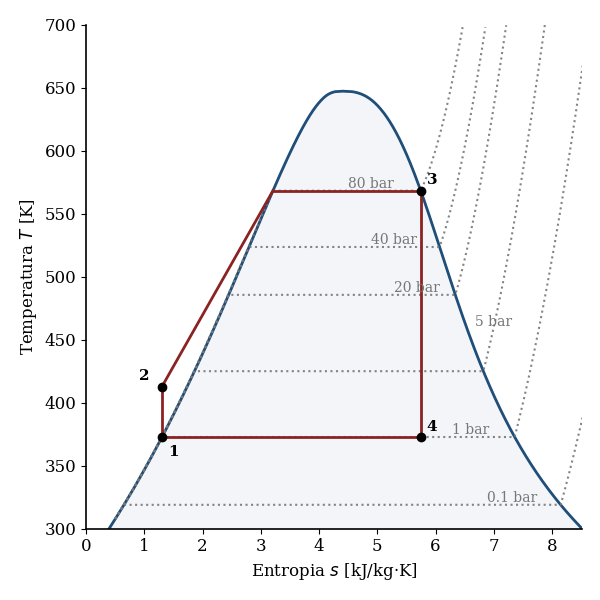
\includegraphics[width=0.45\linewidth]{graphs/rankine-Ts-ideal-ideal.png}
    \caption{Ciclo de Rankine Ideal}
    \label{fig:rankine-Ts-ideal-ideal}
\end{figure}

\subsection{Ciclo de Rankine Sobreaquecido}

De forma semelhante à compressão, durante a expansão na turbina a presença de gotas de água diminui a eficiência da turbina e aumenta a necessidade de manutenção da turbina, pelo que é comum manter a qualidade na saída da turbina ser de pelo menos $90 \%$.

Por outro lado, estamos a aumentar a temperatura média de adição de calor $\bar{T}_H$, pelo que a eficiência térmica do ciclo aumenta.

Para isso, é necessário aquecer mais a água, aumentando $T_3$. É de notar que aumentando a temperatura também aumenta $v$, pelo que o trabalho gerado na turbina será maior. De igual forma, sendo as isobáricas divergentes, o rácio $\frac{Q_C}{Q_H}$ diminui, aumentando a eficiência do ciclo.

Assim, de um ponto de vista teórico, o ideal seria que o fluido saísse da turbina com título $x=1$, i.e. vapor saturado, tal como na Figura \ref{fig:rankine-Ts-ideal-sobreaquecido}, havendo menor condensação e menor erosão mecânica das pás por impacto de gotículas de água. No entanto, na engenharia prática, tal não é viável.

\begin{figure}[H]
    \centering
    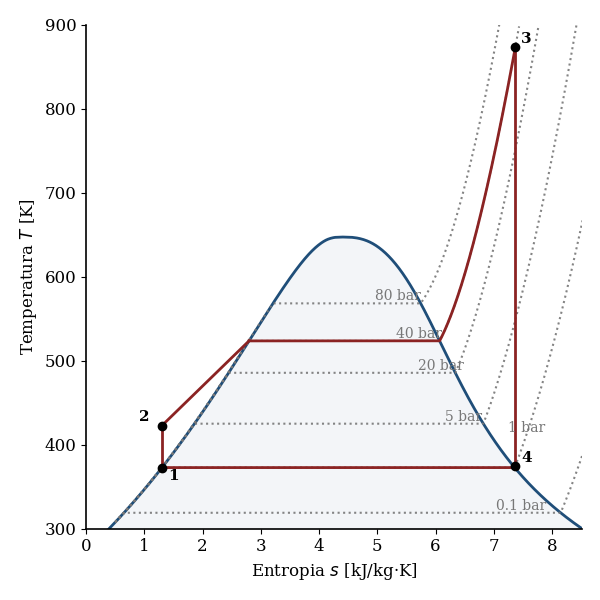
\includegraphics[width=0.45\textwidth]{graphs/rankine-Ts-ideal-sobreaquecido.png}
    \caption{Ciclo de Rankine Sobreaquecido}
    \label{fig:rankine-Ts-ideal-sobreaquecido}
\end{figure}

Um exemplo de um Ciclo de Rankine é uma central de produção de energia elétrica, representada na Figura \ref{fig:rankine-Ts-ideal-powerplant}, que trabalha entre $0.1~\text{bar}$ e $80~\text{bar}$ com uma temperatura máxima de $773.15~\text{K}$ e $319~\text{K}$ de mínima: 

\begin{figure}[H]
    \centering
    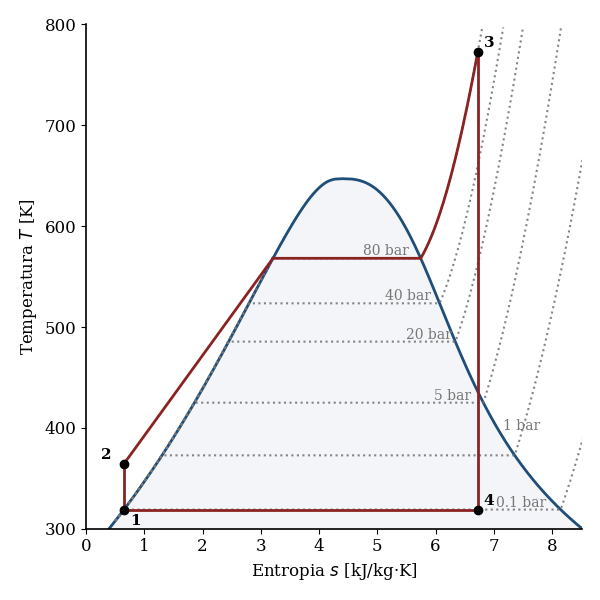
\includegraphics[width=0.45\linewidth]{graphs/rankine-Ts-ideal-powerplant.png}
    \caption{Ciclo de Rankine de uma Central Elétrica}
    \label{fig:rankine-Ts-ideal-powerplant}
\end{figure}

Na verdade, o estado 2, após a compressão na bomba está exagerado, dado que, em condições ideais, a temperatura da água aumentaria apenas cerca de $0.268~\text{K}$. O gráfico à escala está representado na Figura \ref{fig:rankine-Ts-ideal-true-powerplant}. Na Figura \ref{fig:rankine-pump-amp}, pode-se observar a proximidade das isobáricas à curva da água líquida saturada. Esta proximidade evidencia a facilidade (baixo trabalho) em comprimir água líquida, devido ao baixo volume específico. Recordando $(\frac{\dot{W}}{\dot{m}} = \int v dp)$

\begin{figure}[H]
    \centering
    \begin{subfigure}{0.45\textwidth}
        \centering
        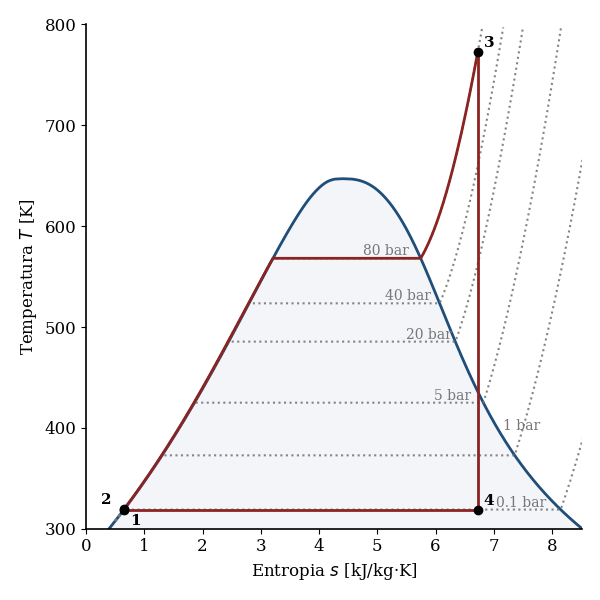
\includegraphics[width=\textwidth]{graphs/rankine-Ts-ideal-true-powerplant.png}
        \caption{Ciclo de Rankine à escala}
        \label{fig:rankine-Ts-ideal-true-powerplant}
    \end{subfigure}
    \hfill
    \begin{subfigure}{0.4\textwidth}
        \centering
        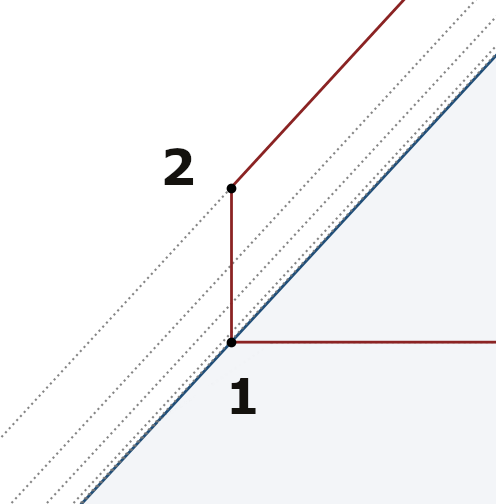
\includegraphics[width=\textwidth]{graphs/pump-amp.png}
        \caption{Ampliação do Processo de Compressão}
        \label{fig:rankine-pump-amp}
    \end{subfigure}
    \caption{Compressão à escala real}
\end{figure}

Considerando cada componente que compõe o ciclo isoladamente e aplicando o balanço de energia, podemos obter o trabalho e o calor específicos de cada componente.

Pode-se notar que o módulo destas quantidades é sempre dado pela diferença de entalpia entre o ponto onde o fluido circulante tem maior entalpia e o ponto onde esta é menor. Por exemplo, na bomba o fluido terá mais energia (entalpia) após a compressão, logo, considerando a compressão um processo adiabático:

\begin{eqnarray*}
    \cancelto{0}{\frac{dE}{dt}} = \cancelto{0}{\dot{Q}} + \dot{W_b} + \dot{m} (h_1 - h_2) \\
    \frac{\dot{W}_b}{\dot{m}} = h_2 - h_1
\end{eqnarray*}

\begin{itemize}
    \item \textbf{Processo 1 $\rightarrow$ 2 (Bomba):} $\frac{\dot{W}_b}{\dot{m}} = h_2 - h_1$
    \item \textbf{Processo 2 $\rightarrow$ 3 (Caldeira):} $\frac{\dot{Q}_H}{\dot{m}} = h_3 - h_2$
    \item \textbf{Processo 3 $\rightarrow$ 4 (Turbina):} $\frac{\dot{W}_t}{\dot{m}} = h_3 - h_4$
    \item \textbf{Processo 4 $\rightarrow$ 1 (Condensador):} $\frac{\dot{Q}_C}{\dot{m}} = h_4 - h_1$
\end{itemize}

No caso da bomba, sendo água líquida, também podemos calcular o trabalho para um processo internamente reversível, por (tal como visto em \ref{eq:w-intrev}):

\begin{equation}
    \left( \frac{\dot{W}_b}{\dot{m}} \right)_{\substack{\text{int} \\ \text{rev}}} = \int v dp \approx v (p_2 - p_1)
\end{equation}

que é, na verdade, a mesma expressão, pois processos internamente reversíveis e adiabáticos (que são as condições, tanto na bomba, como na turbina no ciclo de Rankine ideal) são isentrópicos, e da Equação \ref{eq:2tds} (válida para processos internamente reversíveis) temos: $dh = \cancelto{0}{Tds} + vdp \implies dh = vdp$.

\subsection{Ciclo de Rankine Real}

Considerando que a bomba e a turbina não são ideais, obtemos uma representação de um ciclo real, como a da Figura \ref{fig:rankine-Ts-real-powerplant}, sem considerar perdas de pressão nas tubagens.

\begin{figure}[H]
    \centering
    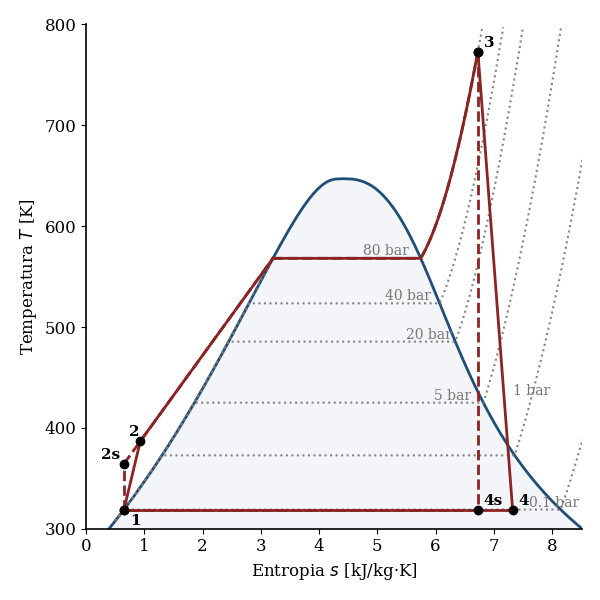
\includegraphics[width=0.45\linewidth]{graphs/rankine-Ts-real-powerplant.png}
    \caption{Ciclo de Rankine Real}
    \label{fig:rankine-Ts-real-powerplant}
\end{figure}

Pode-se pensar que, na bomba, o ideal é fornecer o menor trabalho possível que na mesma atinja o objetivo. Desta forma, o trabalho isentrópico (sem irreversibilidades) será menor que o trabalho real, onde se gera entropia.

Por isso, a \textbf{eficiência isentrópica} do compressor é dada por:

\begin{equation}
    \eta_b = \frac{(\dot{W}_b/\dot{m})_s}{(\dot{W}_b/\dot{m})} = \frac{h_{2s} - h_1}{h_{2} - h_1}
\end{equation}

Por outro lado, na turbina o caso ideal é quando recebemos o maior trabalho possível e, portanto, o trabalho isentrópico será maior que o trabalho real:

\begin{equation}
    \eta_t = \frac{(\dot{W}_t/\dot{m})}{(\dot{W}_t/\dot{m})_s} = \frac{h_3 - h_4}{h_3 - h_{4s}}
\end{equation}

Como o trabalho da bomba é muito menor que o trabalho da turbina, as irreversibilidades na bomba têm normalmente um impacto menor na eficiência térmica do que as da turbina. A maior fonte de irreversibilidade está associada à combustão e a transferência de calor dos produtos de combustão para o fluido circulante.

A eficiência do ciclo de Rankine é:

\begin{equation}
    \eta = \frac{W_t - W_c}{Q_H} = \frac{h_3 - h_4 - (h_2 - h_1)}{h_3 - h_2} = 1 - \frac{h_4 - h_1}{h_3 - h_2} = 1 - \frac{T_4 - T_1}{T_3 - T_2} 
\end{equation}

Comparando com a eficiência máxima de Carnot:

\begin{equation*}
    \eta = \frac{Q_H - Q_c}{Q_H} = 1 - \frac{Q_c}{Q_H} = 1 - \frac{\frac{\dot{Q}_C}{\dot{m}}}{\frac{\dot{Q}_H}{\dot{m}}} = 1 -\frac{T_C (s_{4s} - s_1)}{\bar{T}_H (s_3 - s_{2s})} = 1 -\frac{T_C}{\bar{T}_H}
\end{equation*}

Como a temperatura média $\bar{T}_H$ de adição de calor na fonte quente é inferior a $T_H$, o ciclo de Rankine ideal tem uma eficiência menor que o ciclo de Carnot ideal entre as mesmas fontes. Assim, a eficiência do ciclo tende a aumentar com o aumento de $\bar{T}_H$ e/ou a diminuição de $\bar{T}_C$.



\section{Ciclo de Brayton}

O Ciclo de Brayton faz parte de ciclo de turbinas a gás. Considera-se como fluido circulante do ciclo ar como gás perfeito. Na expansão isotérmica de 4 para 1, não está conectado, pois muitas vezes o ar é expelido para a atmosfera em 4 na mesma pressão e a uma temperatura superior à de entrada em 1.

O ciclo opera entre duas pressões: a de entrada e saída, $p_1$, e a pressão de trabalho $p_2$ ($p_2 > p_1$). A razão de pressão é definida como: $r_p = \frac{p_2}{p_1} = \frac{p_3}{p_4}$.

Normalmente, é sabido $p_1$, $T_1$, ambiente, e $T_3$, após a combustão e condicionado por limitações físicas dos materiais das turbinas.

Para gás perfeito temos $\Delta s = c_p \ln \frac{T}{T_0} - R \ln \frac{p}{p_0}$, pelo que as isobáricas são exponenciais: $T = T_0 e^{\frac{\Delta s + R \ln \frac{p}{p_0}}{c_p}}$

\begin{figure}[H]
    \centering
    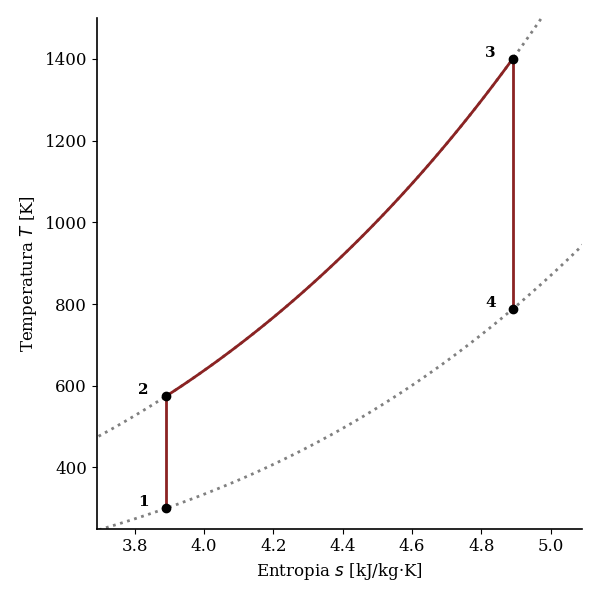
\includegraphics[width=0.45\linewidth]{graphs/brayton-Ts-ideal.png}
    \caption{Ciclo de Brayton Ideal}
    \label{fig:brayton-Ts-ideal}
\end{figure}

\begin{itemize}
    \item \textbf{Processo 1 $\rightarrow$ 2 (Compressor):} $\frac{\dot{W}_c}{\dot{m}} = h_2 - h_1$
    \item \textbf{Processo 2 $\rightarrow$ 3 (Combustão):} $\frac{\dot{Q}_H}{\dot{m}} = h_3 - h_2$
    \item \textbf{Processo 3 $\rightarrow$ 4 (Turbina):} $\frac{\dot{W}_t}{\dot{m}} = h_3 - h_4$
\end{itemize}

Neste exemplo, $T_1 = 300~\text{K}$, $T_3 = 1400~\text{K}$ e $p_1 = 1~\text{bar}$, $r_p = 10$, pelo que $p_2 = 10~\text{bar}$.

Como são processos isentrópicos $\frac{T_2}{T_1} = \left( \frac{p_2}{p_1} \right)^{(k-1)/k}$, podemos obter as temperaturas:

\begin{eqnarray}
    T_2 = T_1 \left( \frac{p_2}{p_1} \right)^{(k-1)/k} = T_1 \left( r_p \right)^{(k-1)/k} \\
    T_4 = T_3 \left( \frac{p_4}{p_3} \right)^{(k-1)/k} = T_3 \left( \frac{1}{r_p} \right)^{(k-1)/k}
\end{eqnarray}

A eficiência do Ciclo de Brayton é:

\begin{equation*}
    \eta = \frac{W_t - W_c}{Q_H} = \frac{h_3 - h_4 - (h_2 - h_1)}{h_3 - h_2} = 1 - \frac{h_4 - h_1}{h_3 - h_2} = 1 - \frac{T_4 - T_1}{T_3 - T_2} = 1 - \frac{T_1 \left(\frac{T_4}{T_1} -1\right)}{T_2 \left(\frac{T_3}{T_2} -1\right)}
\end{equation*}

Como

\begin{equation*}
    r_p = \frac{p_2}{p_1} = \frac{p_3}{p_4} \implies \frac{T_2}{T_1} = \frac{T_3}{T_4} \implies \frac{T_4}{T_1} = \frac{T_3}{T_2}
\end{equation*}

concluimos, então, que a eficiência do ciclo é:

\begin{equation}
    \eta = 1 - \frac{T_1}{T_2} = 1 - \left(\frac{1}{r_p}\right)^{(k-1)/k}
\end{equation}

Esta é a eficiência máxima de um Ciclo de Brayton real, substituindo $T_2$ por $T_{2s}$. A eficiência real do ciclo tem de ser calculado por $\eta = \frac{W_t - W_c}{Q_H} = 1 - \frac{h_4 - h_1}{h_3 - h_2} = 1 - \frac{T_4 - T_1}{T_3 - T_2}$. 

Podemos ver que a eficiência no Ciclo de Brayton Ideal, a eficiência do ciclo depende somente da razão de pressão e, por isso, do estágio de compressão. Quanto maior a razão de pressão, maior a eficiência.

\subsection{Trabalho máximo}

Podemos ver qual a razão de pressão ótima, tal que o trabalho útil é máximo.

A razão de pressão é máxima quando aumentamos $p_2 \to p_{max}$, no limite só podemos aumentar esta até que $T_2 \to T_3$, pelo que $r_{p_{max}} = \frac{p_{max}}{p_1} = \left(\frac{T_3}{T_1}\right)^{k/(k-1)}$

O trabalho útil é:

\begin{equation*}
    \dot{W}_u = \dot{W}_t - \dot{W}_c = h_3 - h_4 - (h_2 - h_1) = \dot{m} c_p (T_3 - T_4) - \dot{m} c_p (T_2 - T_1)
\end{equation*}

Dividindo para obter o trabalho específico e simplificar os cálculos:

\begin{equation*}
\begin{split}
    \frac{\dot{W}_u}{\dot{m} c_p T_1} & = \frac{T_3}{T_1} \left(1 - \frac{T_4}{T_3}\right) - \left(\frac{T_2}{T_1}-1\right)\\
    & = (r_{p_{max}})^{(k-1)/k} \left(1 - \left(\frac{1}{r_p}\right)^{(k-1)/k}\right) - \left((r_p)^{(k-1)/k} -1 \right)
\end{split}
\end{equation*}

Para encontrar o máximo, derivamos e igualamos a zero para encontraro ponto de máximo:

\begin{equation*}
\begin{split}
    \frac{\partial}{\partial r_p} \left( \frac{\dot{W}_u}{\dot{m} c_p T_1} \right) = 0 \Longleftrightarrow &  (r_{p_{max}})^{(k-1)/k} \frac{k-1}{k} \left(\frac{1}{r_p} \right)^{-1/k} \frac{1}{r_p^2} - \frac{k-1}{k} (r_p)^{-1/k} = 0 \\
    & (r_{p_{max}})^{(k-1)/k} \left(\frac{1}{r_p} \right)^{-1/k} \frac{1}{r_p^2} = (r_p)^{-1/k} \\
    & (r_{p_{max}})^{(k-1)/k} = (r_p)^{2-2/k} \Longleftrightarrow (r_{p_{max}})^{(k-1)/k} = (r_p)^{2(k-1)/k}
\end{split}
\end{equation*}

Assim,
\begin{equation}
    r_p = \sqrt{r_{p_{max}}} = \sqrt{\left(\frac{T_3}{T_1}\right)^{k/(k-1)}} = \left(\frac{T_3}{T_1}\right)^{k/[2(k-1)]}
\end{equation} 

Normalmente, é desejável aumentar a eficiência do ciclo, o que implica aumentar a razão de pressão. No entanto, se se ultrapassar a razão de pressão ótima, o trabalho específico útil do ciclo diminuirá. Caso se queira manter a potência útil do ciclo para uma eficiência que implica uma razão de pressão superior ao ponto ótimo: $\sqrt{r_{p_{max}}}$, será necessário aumentar o caudal mássico, $\dot{m}$.

\subsection{Ciclo de Brayton Real}

\begin{figure}[H]
    \centering
    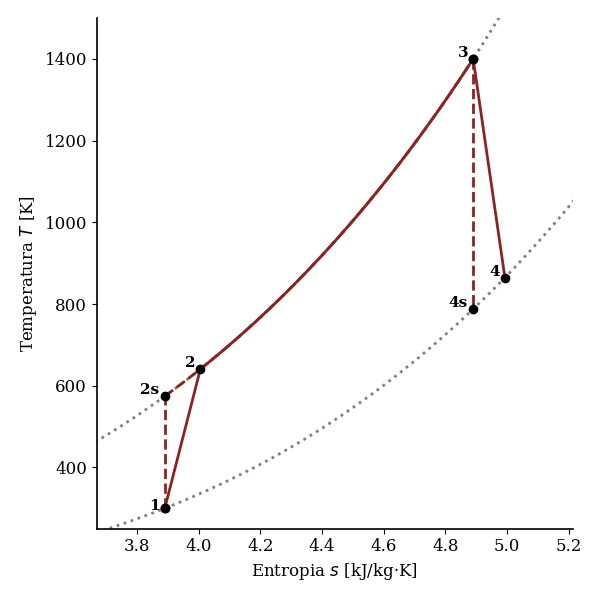
\includegraphics[width=0.45\linewidth]{graphs/brayton-Ts-real.png}
    \caption{Ciclo de Brayton Real}
    \label{fig:brayton-Ts-real}
\end{figure}

No caso real, temos de considerar as irreversibilidades no compressor e na turbina, que terão eficiências isentrópicas, respetivamente, $\eta_c$ e $\eta_t$.

Pode-se pensar que, no compressor, o ideal é fornecer o menor trabalho possível que atinja o objetivo, desta forma o trabalho isentrópico (sem irreversibilidades) será menor que o trabalho real, onde se gera entropia.

Por isso, a eficiência isentrópica do compressor é dado por:

\begin{equation}
    \eta_c = \frac{(\dot{W}_c/\dot{m})_s}{(\dot{W}_c/\dot{m})} = \frac{h_{2s} - h_1}{h_{2} - h_1}
\end{equation}

Por outro lado, na turbina o caso ideal é onde recebemos o maior trabalho possível e, portanto, o trabalho isentrópico será maior que o trabalho real:

\begin{equation}
    \eta_t = \frac{(\dot{W}_t/\dot{m})}{(\dot{W}_t/\dot{m})_s} = \frac{h_3 - h_4}{h_3 - h_{4s}}
\end{equation}

Assim, sabendo as eficiências isentrópicas pode-se calcular os estados reais, normalmente, desconhecidos através de $h_2$ e $h_4$.

Além disso, sendo gás perfeito, temos $h= c_p T$:

\begin{equation}
    \eta_c = \frac{T_{2s} - T_1}{T_{2} - T_1} \qquad \eta_t = \frac{T_3 - T_4}{T_3 - T_{4s}}
\end{equation}

E podemos calcular as incógnitas $T_2$ e $T_4$:

\begin{equation}
    T_2 = T_1 + \frac{T_{2s} - T_1}{\eta_c} \qquad T_4 = T_3 + \eta_t (T_{4s} - T_3) 
\end{equation}

Sendo a eficiência máxima dada por:

\begin{equation}
    \eta_{max} = 1 - \frac{T_1}{T_{2s}} = 1 - \left(\frac{1}{r_p}\right)^{(k-1)/k}
\end{equation}

\subsection{Arrefecimento por andares - Intercooling}

Usando arrefecimento por andares, ou intercooling, consegue-se reduzir o trabalho específico de compressão necessário: $(\dot{W}/\dot{m}) = \int vdp$, pois a menor temperatura, menor o volume específico $v = \frac{RT}{p}$, para a mesma pressão.
Para se atingir esse objetivo, substitui-se o compressor por um dado número de compressores intercalados por radiadores, para arrefecer o ar entre compressões.

No caso de dois compressores dispostos em série — series twin-turbo — o ar é primeiro comprimido até uma pressão intermediária pelo primeiro turbo, depois arrefecido num intercooler, e finalmente comprimido até à pressão final pelo segundo turbo. Idealmente, com múltiplos estágios de compressão e arrefecimento perfeito entre eles, seria possível atingir a pressão final mantendo a temperatura aproximadamente constante, aproximando-se de uma compressão isotérmica (processo $pv=\text{const.}$ para gás ideal), que é mais eficiente do ponto de vista termodinâmico.

\begin{figure}[H]
    \centering
    \begin{subfigure}{0.4\textwidth}
        \centering
        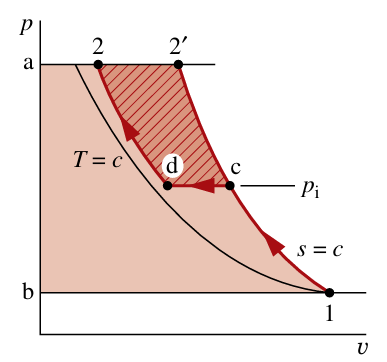
\includegraphics[width=\textwidth]{images/intercooling.png}
        \caption{Compressão em dois estágios com intercooling - Diagrama p-v \cite{shapiro}}
        \label{fig:intercooling}
    \end{subfigure}
    \hfill
    \begin{subfigure}{0.4\textwidth}
        \centering
        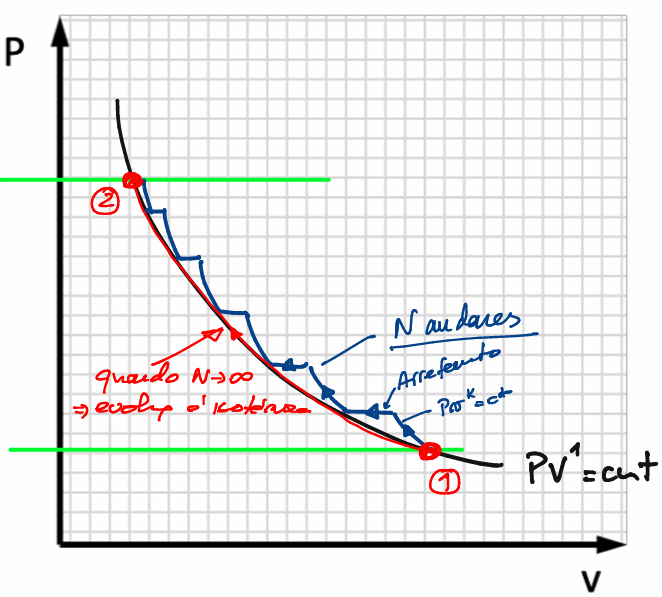
\includegraphics[width=\textwidth]{images/intercooling-isotermico.png}
        \caption{Intercooling ideal - processo isotérmico}
        \label{fig:intercooling-isotermico}
    \end{subfigure}
    \caption{Intercooling - Diagramas p-v}
\end{figure}

Como $\frac{\dot{W}}{\dot{m}} = \int v dp$, o trabalho é a área entre as linhas dos processos $pv^n = \text{const.}$ e o eixo $p$ (pressão) limitado pelas duas linhas horizontais referentes à pressão inicial e final ($p_1$ e $p_2$).

Assim, há uma diminuição do trabalho necessário de compressão necessário entre $p_1$ e $p_2$ ao se arrefecer em estágios intermédios. Além disso, pode-se ver que a área é mínima para o processo isotérmico.


\begin{figure}[H]
    \centering
    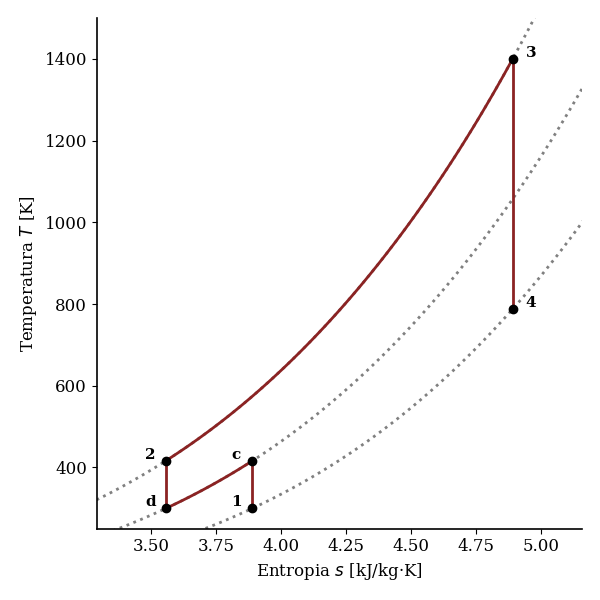
\includegraphics[width=0.45\linewidth]{graphs/brayton-Ts-ideal-intercooling.png}
    \caption{Compressão em dois estágios com intercooling - Diagrama T-s}
    \label{fig:brayton-Ts-ideal-intercooling}
\end{figure}

A pressão intermédia ótima, onde o trabalho de compressão é mínimo, para esta configuração pode ser calculada:

\begin{equation*}
    \frac{\dot{W}}{\dot{m}} = (h_c - h_1) + (h_2 - h_d)
\end{equation*}

onde há uma primeira compressão de 1 para c, arrefecimento de c para d e compressão final de d para 2.

\begin{equation*}
    \frac{\dot{W}}{\dot{m}} = c_p(T_c - T_1) + c_p(T_2 - T_d) = c_p T_1\left(\frac{T_c}{T_1} - 1\right) + c_p T_d \left(\frac{T_2}{T_d} - 1 \right)
\end{equation*}

Considerando compressão isentrópica: $\frac{T_c}{T_1} = \left( \frac{p_i}{p_1} \right)^{(k-1)/k}$ e $\frac{T_2}{T_d} = \left( \frac{p_2}{p_i} \right)^{(k-1)/k}$

\begin{equation*}
    \frac{\dot{W}}{\dot{m}} = c_p T_1\left(\left( \frac{p_i}{p_1} \right)^{(k-1)/k} - 1\right) + c_p T_d \left(\left( \frac{p_2}{p_i} \right)^{(k-1)/k} - 1 \right)
\end{equation*}

\begin{equation*}
    \begin{split}
        \frac{\partial (\dot{W}/ \dot{m})}{\partial p_i} & = c_p T_1 \left( \frac{k-1}{k} \right) \left[ \left( \frac{p_i}{p_1} \right)^{-1/k}  \left( \frac{1}{p_1} \right) - \frac{T_d}{T_1} \left( \frac{p_2}{p_i} \right)^{-1/k} \left( \frac{p_2}{p_i^2} \right) \right] \\
        & = c_p T_1 \left( \frac{k-1}{k} \right) \frac{1}{p_i} \left[ \left( \frac{p_i}{p_1} \right)^{(k-1)/k} - \frac{T_d}{T_1} \left( \frac{p_2}{p_i} \right)^{(k-1)/k} \right]
    \end{split}
\end{equation*}

\begin{eqnarray}
    \frac{\partial (\dot{W}/ \dot{m})}{\partial p_i} = 0 \Longleftrightarrow \left( \frac{p_i}{p_1} \right)^{(k-1)/k} = \frac{T_d}{T_1} \left( \frac{p_2}{p_i} \right)^{(k-1)/k} \nonumber \\ 
    \implies \frac{p_i}{p_1} = \left( \frac{T_d}{T_1}\right)^{k/(k-1)} \frac{p_2}{p_i} \Longleftrightarrow p_i = \sqrt{p_1 p_2 \left( \frac{T_d}{T_1}\right)^{k/(k-1)}}
\end{eqnarray}

Considerando que o arrefecimento permite que $T_d = T_1$, i.e. voltar a comprimir à mesma temperatura, obtemos o valor ótimo de $p_i = \sqrt{p_1 p_2}$.

No caso real, haverá um aumento de entropia na compressão, sendo necessário maior arrefecimento para atingir a pressão desejada a uma temperatura não muito superior à do caso ideal.

\begin{figure}[H]
    \centering
    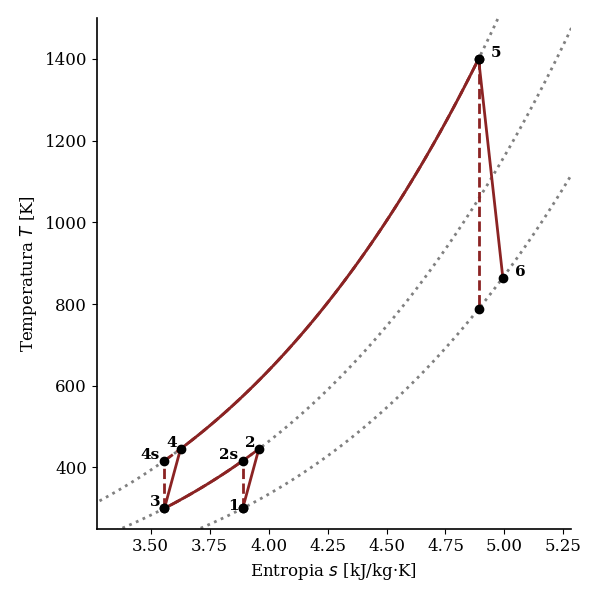
\includegraphics[width=0.45\linewidth]{graphs/brayton-Ts-real-intercooling.png}
    \caption{Ciclo de Brayton Real com Intercooling}
    \label{fig:brayton-Ts-real-intercooling}
\end{figure}